\documentclass[DaoFP]{subfiles}
\begin{document}
\setcounter{chapter}{21}

\chapter{依赖类型}

我们已经见过依赖于其他类型的类型。它们是通过带有类型参数的类型构造器定义的,例如 \hask{Maybe} 或 \hask{[]}。大多数编程语言都对泛型数据类型(即由其他数据类型参数化的数据类型)提供了一定的支持。

从范畴论的角度来看,这些类型被建模为函子\footnote{没有 \hask{Functor} 实例的类型构造器可以视为来自离散范畴的函子——一个除了恒等箭头外没有其他箭头的范畴}。

这一思想的自然推广是让类型由值来参数化。例如,将列表的长度编码在其类型中通常是有优势的。长度为0的列表与长度为1的列表将具有不同的类型,依此类推。

显然,你不能改变这种列表的长度,因为这会改变它的类型。这在函数式编程中不是问题,因为所有数据类型都是不可变的。当你向列表前添加一个元素时,至少在概念上,你创建了一个新列表。对于长度编码的列表,这个新列表具有不同的类型,仅此而已!

由值参数化的类型称为\emph{依赖类型}。有些语言如 Idris 或 Agda 完全支持依赖类型。在 Haskell 中也可以实现依赖类型,但对它们的支持仍然相当零散。

在编程中使用依赖类型的原因是为了使程序可证明正确。为了实现这一点,编译器必须能够检查程序员所做的假设。

Haskell 凭借其强大的类型系统,能够在编译时发现许多错误。例如,除非你为变量的类型提供 \hask{Monoid} 实例,否则它不会让你写 \hask{a <> b}(\hask{mappend} 的中缀表示法)。

然而,在 Haskell 的类型系统中,无法表达或强制执行幺半群的单位元和结合律。为此,\hask{Monoid} 类型类的实例必须携带等式证明(不是实际代码):
\begin{haskell}
assoc :: m <> (n <> p) = (m <> n) <> p
lunit :: mempty <> m = m
runit :: m <> mempty = m
\end{haskell}
依赖类型,特别是等式类型,为实现这一目标铺平了道路。

本章的内容较为高级,且未在本书的其余部分使用,因此你可以在初次阅读时安全地跳过它。此外,为了避免纤维和函数之间的混淆,我决定在本章的部分内容中使用大写字母表示对象。

\section{依赖向量}

我们将从计数列表或向量的标准示例开始:
\begin{haskell}
data Vec n a where
    VNil  :: Vec Z a
    VCons :: a -> Vec n a -> Vec (S n) a
\end{haskell}
如果你包含以下语言编译指示,编译器将识别此定义为依赖类型:
\begin{haskell}
{-# LANGUAGE DataKinds #-}
{-# LANGUAGE GADTs #-}
\end{haskell}
类型构造器的第一个参数是自然数 \hask{n}。注意:这是一个值,而不是一个类型。类型检查器能够从数据构造器中对 \hask{n} 的使用中推断出这一点。第一个构造器创建类型为 \hask{Vec Z a} 的向量,第二个构造器创建类型为 \hask{Vect (S n) a} 的向量,其中 \hask{Z} 和 \hask{S} 被定义为自然数的构造器:
\begin{haskell}
data Nat = Z | S Nat
\end{haskell}

如果我们使用编译指示:
\begin{haskell}
{-# LANGUAGE KindSignatures #-}
\end{haskell}
并导入库:
\begin{haskell}
import Data.Kind
\end{haskell}
我们可以更明确地指定 \hask{n} 是 \hask{Nat},而 \hask{a} 是 \hask{Type}:
\begin{haskell}
data Vec (n :: Nat) (a :: Type) where
    VNil  :: Vec Z a
    VCons :: a -> Vec n a -> Vec (S n) a
\end{haskell}

使用这些定义之一,我们可以构造一个长度为0的(整数)向量:
\begin{haskell}
emptyV :: Vec Z Int
emptyV = VNil
\end{haskell}
它与长度为1的向量具有不同的类型:
\begin{haskell}
singleV :: Vec (S Z) Int
singleV = VCons 42 VNil
\end{haskell}
依此类推。

我们现在可以定义一个依赖类型的函数,返回向量的第一个元素:
\begin{haskell}
headV :: Vec (S n) a -> a
headV (VCons a _) = a
\end{haskell}
该函数保证仅适用于非零长度的向量。这些向量的大小匹配 \hask{(S n)},而 \hask{(S n)} 不能是 \hask{Z}。如果你尝试用 \hask{emptyV} 调用此函数,编译器将标记错误。

另一个例子是将两个向量压缩在一起的函数。其类型签名中编码了要求两个向量具有相同大小 \hask{n}(结果也具有大小 \hask{n}):
\begin{haskell}
zipV :: Vec n a -> Vec n b -> Vec n (a, b)
zipV (VCons a as) (VCons b bs) = VCons (a, b) (zipV as bs)
zipV VNil VNil = VNil
\end{haskell}

依赖类型在编码容器的形状时特别有用。例如,列表的形状编码在其长度中。一个更高级的例子是将树的形状编码为运行时值。

\begin{exercise}
实现函数 \hask{tailV},返回非零长度向量的尾部。尝试用 \hask{emptyV} 调用它。
\end{exercise}

\end{document}

\section{Dependent Types Categorically}

The easiest way to visualize dependent types is to think of them as families of types indexed by elements of a set. In the case of counted vectors, the indexing set would be the set of natural numbers $\mathbb{N}$.

The zeroth type would be the unit type \hask{()} representing an empty vector. The type corresponding to \hask{(S Z)} would be \hask{a}; then we'd have a pair \hask{(a, a)}, a triple \hask{(a, a, a)} and so on, with higher and higher powers of \hask{a}.

If we want to talk about the whole family as one big set, we can take the sum of all these types. For instance, the sum of all powers of $a$ is the familiar list type, a.k.a., a free monoid:
\[ \mathit{List} (a) = 1 + a + a \times a + a \times a \times a + ... =  \sum_{n:\mathbb{N}} a^n \]

\subsection{Fibrations}

Although intuitively easy to visualize, this point of view doesn't generalize nicely to category theory, where we don't like mixing sets with objects. So we turn this picture on its head and instead of talking about injecting family members into the sum, we consider a mapping that goes in the opposite direction. 

This, again, we can first visualize using sets. We have one big set $E$ describing the \emph{entire} family, and a function $p$ called the projection, or a \index{display map}\emph{display map}, that goes from $E$ down to the indexing set $B$ (also called the \emph{base}). 

This function will, in general, map multiple elements to one. We can then talk about the inverse image of a particular element $x \in B$ as the set of elements that get mapped down to it by $p$. This set is called the \index{fiber}\emph{fiber} and is written $p^{-1} x$ (even though, in general, $p$ is not invertible in the usual sense). Seen as a collection of fibers, $E$ is often called a \emph{fiber bundle} or just a bundle.

\[
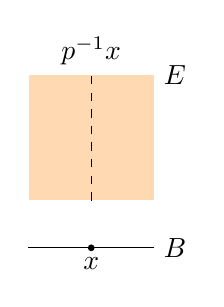
\begin{tikzpicture}

\def\yb{0}; % base
\def\yfb{0.6}; % fiber bottom
\def\yft{2.2}; % fiber top

\def\dx{0.8};

\def\xbl{0};
\def\xbm{\xbl + \dx};
\def\xbr{\xbl + 2*\dx};

\filldraw[fill=orange!30, draw=white] (\xbl, \yfb) rectangle (\xbr, \yft);

\draw (\xbl, \yb) -- (\xbr, \yb);

\draw[dashed] (\xbm, \yfb) -- (\xbm, \yft);

\filldraw[black] (\xbm, \yb) circle (1 pt);
\node[below] at (\xbm, \yb) {$x$};
\node[above] at (\xbm, \yft) {$p^{-1} x$};
\node[right] at (\xbr, \yb) {$B$};
\node[right] at (\xbr, \yft) {$E$};

\end{tikzpicture}
\]


Now forget about sets. A \emph{fibration} in an arbitrary category is a pair of objects $e$ and $b$ and an arrow $p \colon e \to b$. 

So this is really just an arrow, but the context is everything. When an arrow is called a fibration, we use the intuition from sets, and imagine its source $e$ as a collection of fibers, with $p$ projecting each fiber down to a single point in the base $b$. 

We can go even further: since (small) categories form a category $\mathbf{Cat}$ with functors as arrows, we can define a fibration of a category, taking another category as its base. 

\subsection{Type families as fibrations}

We will therefore model type families as fibrations. For instance, our counted-vector family can be represented as a fibration whose base is the type of natural numbers. The whole family is a sum (coproduct) of consecutive powers (products) of $a$:
\[ \mathit{List}(a) = a^0 + a^1 + a^2 + ... = \sum_{n\colon \mathbb{N}} a^n \]
with the zeroth power---the initial object---representing the vector of size zero.
\[
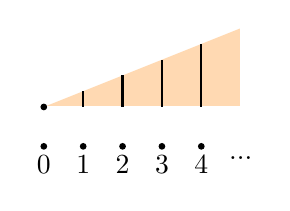
\begin{tikzpicture}
\def\dx{0.5};
\def\yb{0};
\def\dy{0.2};
\def\y{0.5};

\filldraw[fill=orange!30, draw=white] (0, \y) to (5* \dx, \y) to (5*\dx, \y + 5*\dy);

\filldraw[black] (0, 0) circle (1 pt);
\node[below] at (0, 0) {$0$};
\filldraw[black] (0, \y) circle (1 pt);

\filldraw[black] (\dx, 0) circle (1 pt);
\node[below] at (\dx, 0) {$1$};
\draw[thick] (\dx, \y) -- (\dx, \y + \dy);

\filldraw[black] (2*\dx, 0) circle (1 pt);
\node[below] at (2*\dx, 0) {$2$};
\draw[thick] (2*\dx, \y) -- (2*\dx, \y + 2* \dy);

\filldraw[black] (3*\dx, 0) circle (1 pt);
\node[below] at (3*\dx, 0) {$3$};
\draw[thick] (3*\dx, \y) -- (3*\dx, \y + 3* \dy);

\filldraw[black] (4*\dx, 0) circle (1 pt);
\node[below] at (4*\dx, 0) {$4$};
\draw[thick] (4*\dx, \y) -- (4*\dx, \y + 4* \dy);
\node[below] at (5*\dx, 0) {$...$};

\end{tikzpicture}
\]

The projection $p \colon \mathit{List}(a) \to \mathbb{N}$ is the familiar $\mathit{length}$ function. 

In category theory we like to describe things in bulk---defining internal structure of things by structure-preserving maps between them. Such is the case with fibrations. If we fix the base object $b$ and consider all possible source objects in the category $\mathcal{C}$, and all possible projections down to $b$, we get a \emph{slice category} $\mathcal{C}/b$. This category represents all the ways we can slice the objects of $\cat C$ over the base $b$.

Recall that the objects in the slice category are pairs $\langle e, p \colon e \to b \rangle$, and a morphism between two objects $\langle e, p \rangle$ and $\langle e', p' \rangle$ is an arrow $f \colon e \to e'$ that commutes with the projections, that is:
\[p' \circ f = p \]
The best way to visualize this is to notice that such a morphism maps fibers of $p$ to fibers of $p'$. It's a ``fiber-preserving'' mapping between bundles.

\[
 \begin{tikzcd}
 e
 \arrow[rd, "p"']
 \arrow[rr, "f"]
 && e'
 \arrow[ld, "p'"]
 \\
 &b
  \end{tikzcd}
\]

Our counted vectors can be seen as objects in the slice category $\mathcal{C}/\mathbb{N}$ given by pairs $\langle \mathit{List}(a), \mathit{length} \rangle$. A morphism in this category maps vectors of length $n$ to vectors of the same length $n$.

\subsection{Pullbacks}

We've seen a lot of examples of commuting squares. Such a square is a graphical representation of an equation: two path between opposite corners of a square, each a result of a composition of two morphisms, are equal. 

Like with every equality we may want to replace one or more of its components with an unknown, and try to solve the resulting equation. For instance, we may ask the question: Is there an object together with two arrows that would complete a commuting square? If many such objects exist, is there a universal one? If the missing piece of the puzzle is the upper left corner of a square (the source), we call it a pullback. If it's the lower right corner (the target), we call it a \index{pushout}pushout.

\[
 \begin{tikzcd}
 \color{red}?
 \arrow[d, red, dashed, "?"']
 \arrow[r, red, dashed, "?"]
 & E
 \arrow[d, "p"]
 \\
 A
 \arrow[r, "f"]
 &B
\end{tikzcd}
\hspace{40pt}
\begin{tikzcd}
 E
 \arrow[d, "p"']
 \arrow[r, "f"]
 & E'
 \arrow[d, red, dashed, "?"]
 \\
 B
 \arrow[r, red, dashed, "?"]
 &\color{red}?
 \end{tikzcd}
\]


 Let's start with a particular fibration $p \colon E \to B$ and ask ourselves the question: what happens when we change the base from $B$ to some $A$ that is related to it through a mapping $f \colon A \to B$. Can we ``pull the fibers back'' along $f$? 
 
 Again, let's think about sets first. Imagine picking a fiber in $E$ over some point $y \in B$ that is in the image of $f$. If $f$ were invertible, there would be an element $x = f^{-1} y$. We'd plant our fiber over it. In general, though, $f$ is not invertible. It means that there could be more elements of $A$ that are mapped to our $y$. In the picture below you see two such elements, $x_1$ and $x_2$. We'll just duplicate the fiber above $y$ and plant it over all elements that map to $y$. This way, every point in $A$ will have a fiber sticking out of it. The sum of all these fibers will form a new bundle $E'$.
 

\[
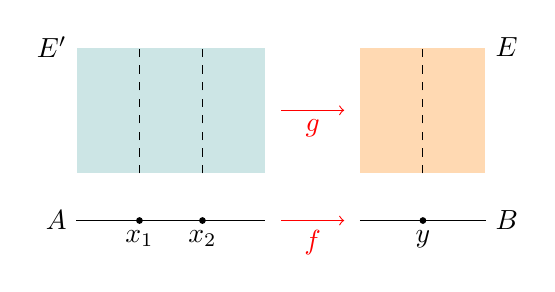
\begin{tikzpicture}

\def\yb{0}; % base
\def\yfb{0.6}; % fiber bottom
\def\yft{2.2}; % fiber top
\def\yfm{1.4} % fiber middle

\def\dx{0.8};

\def\xal{-1.8};
\def\xam{\xal + \dx};
\def\xamm{\xal + 2 * \dx};
\def\xar{\xal + 3*\dx};

\def\xbl{1.8};
\def\xbm{\xbl + \dx};
\def\xbr{\xbl + 2*\dx};

\filldraw[fill=blue!50!green!20, draw=white] (\xal, \yfb) rectangle (\xar, \yft);
\filldraw[fill=orange!30, draw=white] (\xbl, \yfb) rectangle (\xbr, \yft);

\draw (\xal, \yb) -- (\xar, \yb);
\draw (\xbl, \yb) -- (\xbr, \yb);

\draw[dashed] (\xam, \yfb) -- (\xam, \yft);
\draw[dashed] (\xamm, \yfb) -- (\xamm, \yft);
\draw[dashed] (\xbm, \yfb) -- (\xbm, \yft);

\filldraw[black] (\xam, \yb) circle (1 pt);
\filldraw[black] (\xamm, \yb) circle (1 pt);
\filldraw[black] (\xbm, \yb) circle (1 pt);
\node[below] at (\xbm, \yb) {$y$};
\node[right] at (\xbr, \yb) {$B$};
\node[left] at (\xal, \yb) {$A$};
\node[right] at (\xbr, \yft) {$E$};
\node[left] at (\xal, \yft) {$E'$};
\node[below] at (\xam, \yb) {$x_1$};
\node[below] at (\xamm, \yb) {$x_2$};

\draw[->, red] (\xar + 0.2, \yb) -- (\xbl - 0.2, \yb) node [midway, below] {$f$};
\draw[->, red] (\xar + 0.2, \yfm) -- (\xbl - 0.2, \yfm) node [midway, below] {$g$};

\end{tikzpicture}
\]

We have thus constructed a new fibration with the base $A$. Its projection $p' \colon E' \to A$ maps each point in a given fiber to the point over which this fiber was planted. There is also an obvious mapping $g \colon E' \to E$ that maps fibers to their corresponding fibers. 

By construction, this new fibration $\langle E', p'\rangle$ satisfies the condition:
\[ p \circ g = f \circ p' \]
which can be represented as a commuting square:
\[
 \begin{tikzcd}
 E'
 \arrow[d, "p'"']
 \arrow[r, "g"]
 & E
 \arrow[d, "p"]
 \\
 A
 \arrow[r, "f"]
 &B
  \end{tikzcd}
\]

In  $\mathbf{Set}$, we can explicitly construct $E'$ as a \emph{subset} of the cartesian product $A \times E$ with $p' = \pi_1$ and $g = \pi_2$ (the two cartesian projections). An element of $E'$ is a pair $\langle a, e \rangle$, such that:
\[ f (a) = p (e) \]

This commuting square is the starting point for the categorical generalization. However, even in $\mathbf{Set}$ there are many different fibrations over $A$ that make this diagram commute. We have to pick the universal one. Such a universal construction is called a \emph{pullback}, or a \emph{fibered product}.

In category theory, a \index{pullback}pullback of $p \colon e \to b$ along $f \colon a \to b$ is an object $e'$ together with two arrows $p' \colon e' \to a$ and $g \colon e' \to e$ that makes the following diagram commute\[
 \begin{tikzcd}
 &e'
 \arrow[r, "g"]
 \arrow[d, "p'"']
 &e
 \arrow[d, "p"]
 \\
 &a
 \arrow[r, "f"]
 &b
  \end{tikzcd}
\]
and that satisfies the universal condition. 


The universal condition says that, for any other candidate object $x$ with two arrows $q' \colon x \to e$ and $q \colon x \to a$ such that $p \circ q' = f \circ q$ (making the bigger ``square'' commute), there is a unique arrow $h \colon x \to e'$ that makes the two triangles commute, that is:
\begin{align*}
q &= p' \circ h \\
q' &= g \circ h
\end{align*}
Pictorially:
\[
 \begin{tikzcd}
 x
 \arrow[dr, dashed, "h"]
 \arrow[drr, bend left, "q'"]
 \arrow[ddr, bend right, "q"']
 \\
 &e'
 \arrow[r, "g"]
 \arrow[d, "p'"']
\arrow[dr, phantom,  , very near start, "\lrcorner"]
 &e
 \arrow[d, "p"]
 \\
 &a
 \arrow[r, "f"]
 &b
  \end{tikzcd}
\]
The angle symbol in the upper corner of the square is used to mark pullbacks.

If we look at the pullback through the prism of sets and fibrations, $e$ is a bundle over $b$, and we are constructing a new bundle $e'$ out of the fibers taken from $e$. Where we plant these fibers over $a$ is determined by (the inverse image of) $f$. This procedure makes $e'$ a bundle over both $a$ and $b$, the latter with the projection $p \circ g = f \circ p'$. 

The $x$ in this picture is some other bundle over $a$ with the projection $q$. It is simultaneously a bundle over $b$ with the projection $f \circ q = p \circ q'$. The unique mapping $h$ maps the fibers of $x$ given by $q^{-1}$ to fibers of $e'$ given by $p'^{-1}$. 

All mappings in this picture work on fibers. Some of them rearrange fibers over new bases---that's what a pullback does.  Other mappings modify individual fibers---the mapping $h \colon x \to e'$ works like this.

If you think of bundles as containers of fibers, the rearrangements of fibers corresponds to natural transformations, and the modifications of fibers correspond to the action of \hask{fmap}.
 
The universal condition then tells us that $q'$ can be factored into a modification of fibers $h$, followed by the rearrangement of fibers $g$.

It's worth noting that picking the terminal object or the singleton set as the pullback target gives us automatically the definition of the cartesian product:
\[
 \begin{tikzcd}
 b \times e
 \arrow[d, "\pi_1"']
 \arrow[r, "\pi_2"]
\arrow[dr, phantom,  , very near start, "\lrcorner"]
 & e
 \arrow[d, "!"]
 \\
 b
 \arrow[r, "!"]
 &
 1
  \end{tikzcd}
\]

Alternatively, we can think of this picture as planting as many copies of $e$ as there are elements in $b$. We'll use this analogy when we talk about the dependent sum and product.

Notice also that a single fiber can be extracted from a fibration by pulling it back to the terminal object. In this case the mapping $x \colon 1 \to b$ picks an element of the base, and the pullback along it extracts a single fiber $\varphi$:
\[
 \begin{tikzcd}
 \varphi
 \arrow[d, "!"']
 \arrow[r, "g"]
\arrow[dr, phantom,  , very near start, "\lrcorner"]
 & e
 \arrow[d, "p"]
 \\
 1
 \arrow[r, "x"]
 &
 b
  \end{tikzcd}
\]
The arrow $g$ injects this fiber back into $e$. By varying $x$ we can pick different fibers in $e$.

\begin{exercise}
Show that the pullback with the terminal object as the target is the product.
\end{exercise}
\begin{exercise}
Show that a pullback can be defined as a limit of the diagram from a stick-figure category with three objects:
\[ a \rightarrow b \leftarrow c \]
\end{exercise}

\begin{exercise}
Show that a pullback in $\mathcal{C}$ with the target $b$ is a product in the slice category $\mathcal{C}/b$. Hint: Define two projections  as morphisms in the slice category. Use universality of the pullback to show the universality of the product.
\end{exercise}

\subsection{Substitution}

We have two alternative descriptions of dependent types: one as fibrations and another as type families. It's in the latter framework that the pullback along a morphism $f$ can be interpreted as a substitution. When we have a type family $T y$ parameterized by elements $y \colon B$ and we always define a new type family by substituting $f x$ for $y$.

\[
 \begin{tikzcd}
 T (f x)
 & T y
 \\
 x
 \arrow[u, mapsto, ""]
 \arrow[r, mapsto, "f"]
 &y
 \arrow[u, mapsto, ""]
  \end{tikzcd}
\]
The new type family is thus parameterized by different shapes.

\subsection{Dependent environments}
When modeling lambda calculus, we used the objects of a cartesian closed category to serve both as types and environments. An empty environment was modeled as the terminal object (unit type), and we were building more complex environments using products. The order in which we multiply types doesn't matter since the product is symmetric (up to isomorphism).

When dealing with dependent types, we have to take into account that the type we are adding to the environment may depend on the values of the types already present in the environment. As before, we start with an empty environment modeled as the terminal object. 

\subsection{Weakening}

\subsection{Base-change functor}

We used a cartesian closed category as a model for programming. To model dependent types, we need to impose an additional condition: We require the category to be \index{locally cartesian closed category}\emph{locally cartesian closed}. This is a category in which all slice categories are cartesian closed. 

In particular, such categories have all pullbacks, so it's always possible to change the base of any fibration.  Base change induces a mapping between slice categories that is functorial. 

Given two slice categories $\mathcal{C}/b$ and $\mathcal{C}/a$ and an arrow between bases $f \colon b \to a$ the base-change functor $f^* \colon \mathcal{C}/a \to \mathcal{C}/b$ maps a fibration $\langle e, p \rangle$ to the fibration $ f^* \langle e, p \rangle= \langle f^* e, f^* p \rangle$, which is given by the pullback:
\[
 \begin{tikzcd}
f^* e
\arrow[dr, phantom,  , very near start, "\lrcorner"]
 \arrow[d, "f^*p"']
 \arrow[r, "g"]
 & e
 \arrow[d, "p"]
 \\
 b
 \arrow[r, "f"]
 &a
  \end{tikzcd}
\]
Notice that the functor $f^*$ goes in the opposite direction to the arrow $f$.

To visualize the base-change functor let's consider how it works on sets. 
\[
 \begin{tikzcd}
f^* E
\arrow[dr, phantom,  , very near start, "\lrcorner"]
 \arrow[d, "f^*p"']
 \arrow[r, "g"]
 & E
 \arrow[d, "p"]
 \\
 B
 \arrow[r, "f"]
 &A
  \end{tikzcd}
\]
We have the intuition that the fibration $p$ decomposes the set $E$ into fibers over each point of $A$. 

We can think of $f$ as another fibration that similarly decomposes $B$. Let's call these fibers in $B$ ``patches.'' For instance, if $A$ is just a two-element set, then the fibration given by $f$ splits $B$ into two patches. The pullback takes a fiber from $E$ and plants it over the whole patch in $B$. The resulting set $f^*E$ looks like a patchwork, where each patch is planted with clones of a single fiber from $E$.


\[
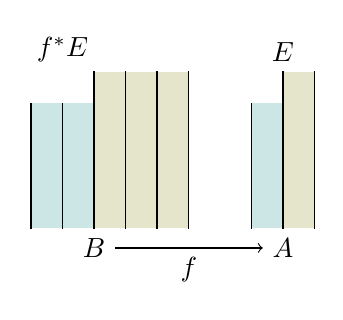
\begin{tikzpicture}
\def\xmin{1.4};
\def\dx{0.4};
\def\xl{-1.4};

\def\dy{0.2};
\def\yb{0};
\def\yt{10 * \dy}; 

% bars over A
\filldraw[fill=blue!50!green!20, draw=white] (\xmin, \yb) rectangle (\xmin + \dx, \yt - 2*\dy);
\filldraw[fill=red!50!green!20, draw=white] (\xmin + \dx, \yb) rectangle (\xmin + 2 * \dx, \yt);

\draw (\xmin, \yb) -- (\xmin, \yt - 2*\dy);
\draw (\xmin + \dx, \yb) -- (\xmin+ \dx, \yt);
\draw (\xmin + 2 * \dx, \yb) -- (\xmin + 2 * \dx, \yt);

\node[below] (BB) at (\xmin + \dx, \yb) {$A$};
\node[above] at (\xmin + \dx, 10 * \dy) {$E$};

% bars over B

\filldraw[fill=blue!50!green!20, draw=white] (\xl, \yb) rectangle (\xl + 5 * \dx, \yt - 2*\dy);
\filldraw[fill=red!50!green!20, draw=white] (\xl + 2*\dx, \yb) rectangle (\xl + 5 * \dx, \yt);
\draw (\xl, \yb) -- (\xl, \yt - 2*\dy);
\draw (\xl + \dx, \yb) -- (\xl + \dx, \yt - 2 * \dy);
\draw (\xl + 2 * \dx, \yb) -- (\xl + 2 * \dx, \yt);
\draw (\xl + 3 * \dx, \yb) -- (\xl + 3 * \dx, \yt);
\draw (\xl + 4 * \dx, \yb) -- (\xl + 4 * \dx, \yt);
\draw (\xl + 5 * \dx, \yb) -- (\xl + 5 * \dx, \yt);

\node[below] (B) at (\xl + 2 * \dx, \yb) {$B$};
\node[above] at (\xl + \dx, 10 * \dy) {$f^* E$};

\draw[->]  (B) -- (BB) node [midway, below] {$f$};


\end{tikzpicture}
\]

Since we have a function from $B$ to $A$ that may map many elements to one, the fibration over $B$ has finer grain than the coarser fibration over $A$. The simplest, least-effort way to turn the fibration of $E$ over $A$ to a fibration over $B$, is to spread the existing fibers over the patches defined by (the inverse of) $f$. This is the essence of the universal construction of the pullback.

In particular, if $A$ is a singleton set (the terminal object), then we have only one fiber (the whole of $E$) and the bundle $f^*E$ is a cartesian product $B \times E$. Such bundle is called a \index{trivial bundle}\emph{trivial bundle}.

A non-trivial bundle is not a product, but it can be \emph{locally} decomposed into products. Just as $B$ is a sum of patches, so $f^*E$ is a sum of products of these patches and the corresponding fibers of $E$.



You may also think of $A$ as providing an \emph{atlas} that enumerates all the patches in the \emph{base} $B$. Imagine that $A$ is a set of countries and $B$ is a set of cities. The mapping $f$ assigns a country to each city.

Continuing with this example, let $E$ be the set of languages fibrated by the country. If we assume that in each city the language of the given country is spoken, the base-change functor replants the country's languages over each of its cities.

By the way, this idea of using local patches and an atlas goes back to differential geometry and general relativity, where we often glue together local coordinate systems to describe topologically nontrivial bundles, like M\"{o}bius strips or Klein bottles.

As we'll see soon, in a locally cartesian closed category, the base change functor has both the left and the right adjoints. The left adjoint to $f^*$ is called $f_!$ (sometimes pronounced ``f down-shriek'') and the right adjoint is called $f_*$ (``f down-star''):
\[ f_! \dashv f^* \dashv f_* \]
In programming, the left adjoint is called the dependent sum, and the right adjoint is called the dependent product or dependent function:
\[ \Sigma_f \dashv f^* \dashv \Pi_f \]

\begin{exercise}
Define the action of the base-change functor on morphisms in $\cat C/a$, that is, given a morphism $h$ construct its counterpart $f^* h$
\[
 \begin{tikzcd}
f^* e'
 \arrow[dr, "f^*p'"']
 \arrow[r, red, "f^* h"]
 & f^* e
\arrow[d, "f^*p"]
&& e'
\arrow[d, "p'"]
\arrow[r, red, "h"]
& e
\arrow[dl, "p"]
 \\
& b
\arrow[rr, "f"']
 &&a
\end{tikzcd}
\hspace{40pt}
\begin{tikzcd}
\end{tikzcd}
\]
Hint: Use the universality of the pullback and the commuting condition: $g' \circ h \circ p = f^* p' \circ f$.

\[
\begin{tikzcd}
 f^* e'
 \arrow[dr, dashed, red, "f^* h"]
 \arrow[drr, bend left, "g' \circ h"]
 \arrow[ddr, bend right, "f^* p'"']
 \\
 &f^* e
 \arrow[r, "g"]
 \arrow[d, "f^* p"']
\arrow[dr, phantom,  , very near start, "\lrcorner"]
 &e
 \arrow[d, "p"]
 \\
 &b
 \arrow[r, "f"]
 &a
\end{tikzcd}
\hspace{40pt}
\begin{tikzcd}
f^* e'
\arrow[r, "g'"]
\arrow[d, "f^* p'"']
\arrow[dr, phantom,  , very near start, "\lrcorner"]
& e'
\arrow[d, "p'"']
\arrow[r, red, "h"]
& e
\arrow[dl, "p"]
\\
b
\arrow[r, "f"]
& a
\end{tikzcd}
\]


\end{exercise}



\section{依赖和 (Dependent Sum)}

在类型论中,依赖和(dependent sum),或称为 $\Sigma$ 类型 $\Sigma_{x : B} T(x)$,被定义为一类对(pair),其中第二个分量的\emph{类型}依赖于第一个分量的\emph{值}。

从概念上讲,和类型(sum type)是通过其映射外性质(mapping-out property)定义的。和的映射外是一对映射,如下伴随关系所示:
\[ \mathcal{C}(F_1 + F_2, F) \cong (\mathcal{C} \times \mathcal{C}) (\langle F_1, F_2 \rangle, \Delta F) \]
这里,我们有一对箭头 $(F_1 \to F, F_2 \to F)$,它们定义了和 $S = F_1 + F_2$ 的映射外。在 $\Set$ 中,和是一个带标签的并集(tagged union)。依赖和则是被另一个集合的元素标记的和。

我们的计数向量类型可以被视为被自然数标记的依赖和。该类型的一个元素是一个自然数 \hask{n}(一个值)与一个 n 元组类型 \hask{(a, a, ... a)} 的元素配对。以下是一些用这种表示法写的整数计数向量:
\begin{haskell}
(0, ())
(1, 42)
(2, (64, 7))
(5, (8, 21, 14, -1, 0))
\end{haskell}

更一般地,依赖和的引入规则假设存在一个由基类型 $B$ 的元素索引的类型族 $T(x)$。然后,$\Sigma_{x : B} T(x)$ 的一个元素由一对元素 $x \colon B$ 和 $y \colon T(x)$ 构造而成。

在范畴论中,依赖和被建模为基变换函子(base-change functor)的左伴随。

为了理解这一点,让我们首先回顾一下对(pair)的定义,它是积(product)的一个元素。我们之前注意到,积可以写成从单元素集(终端对象)的回拉(pullback)。以下是积/回拉的泛构造(universal construction)(符号预示了该构造的目标):
\[
 \begin{tikzcd}
 S
 \arrow[dr, blue, dashed, "\phi^T"]
 \arrow[drr, blue, bend left, "\phi"]
 \arrow[ddr, bend right, "q"]
 \\
 &B \times F
\arrow[dr, phantom,  , very near start, "\lrcorner"]
 \arrow[r, "\pi_2"]
 \arrow[d, "\pi_1"']
 &F
 \arrow[d, "!"]
 \\
 &B
 \arrow[r, "!"]
 &1
  \end{tikzcd}
\]

我们还看到,积可以使用伴随关系来定义。我们可以在图中发现这个伴随关系:对于每对箭头 $\langle \phi, q \rangle$,存在一个唯一的箭头 $\phi^T$,使得三角形交换。

注意,如果我们固定 $q$,我们会得到箭头 $\phi$ 和 $\phi^T$ 之间的一一对应关系。这将是我们感兴趣的伴随关系。

现在,我们可以戴上纤维化(fibration)的眼镜,注意到 $\langle S, q\rangle$ 和 $\langle B \times F, \pi_1 \rangle$ 是同一基 $B$ 上的两个纤维化。交换三角形使得 $\phi^T$ 成为切片范畴 $\mathcal{C}/B$ 中的一个态射,或称为纤维映射(fiber-wise mapping)。换句话说,$\phi^T$ 是以下 hom-集的一个成员:
 \[ (\mathcal{C}/B) \left(\left \langle {S \atop q} \right \rangle, \left \langle {B \times F \atop \pi_1} \right \rangle \right)  \]
 
 由于 $\phi$ 是 hom-集 $ \mathcal{C}(S, F)$ 的一个成员,我们可以将 $\phi^T$ 和 $\phi$ 之间的一一对应关系重写为 hom-集的同构:
\[  (\mathcal{C}/B)\left(\left \langle {S \atop q} \right \rangle, \left \langle {B \times F \atop \pi_1} \right \rangle \right) \cong \mathcal{C}(S, F) \]
事实上,这是一个伴随关系,其中我们有遗忘函子(forgetful functor)$U \colon \mathcal{C}/B \to \mathcal{C}$,将 $\langle S, q \rangle$ 映射到 $S$,从而忘记了纤维化。

如果你仔细观察这个伴随关系,你可以看到 $S$ 作为范畴和(categorical sum,余积)的定义轮廓。

首先,在右边,你有一个从 $S$ 的映射。将 $S$ 视为由纤维化 $\langle S, q \rangle$ 定义的纤维的和。

其次,回想一下,纤维化 $\langle B \times F, \pi_1 \rangle$ 可以被视为在 $B$ 中的点上种植多个 $F$ 的副本。这是对角函子(diagonal functor)$\Delta$ 的推广,它复制 $F$——在这里,我们制作了 $F$ 的“$B$ 个副本”。伴随关系的左边只是一堆箭头,每个箭头将 $S$ 的不同纤维映射到目标纤维 $F$。

\[
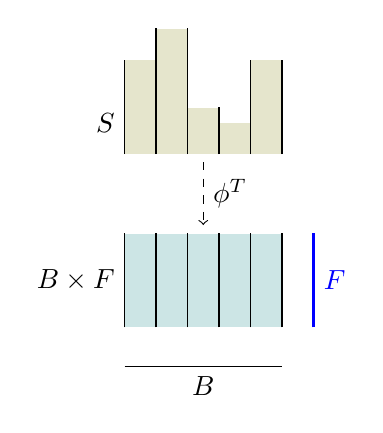
\begin{tikzpicture}
\def\xmin{1.4};
\def\dx{0.4};
\def\xl{-1.4};

\def\dy{0.2};
\def\yb{0.2};
\def\yt{10 * \dy}; 

\def\ybb{-2};
\def\ytt{\ybb + 6 * \dy};

\def\ybase{-2.5}

% bars above

\def\yya{\yt - 3 * \dy}
\def\yyb{\yt - 1 * \dy}
\def\yyc{\yt - 6 * \dy}
\def\yyd{\yt - 7 * \dy}

\filldraw[fill=red!50!green!20, draw=white] (\xl + 0*\dx, \yb) rectangle (\xl + 1 * \dx, \yya);
\filldraw[fill=red!50!green!20, draw=white] (\xl + 1*\dx, \yb) rectangle (\xl + 2 * \dx, \yyb);
\filldraw[fill=red!50!green!20, draw=white] (\xl + 2*\dx, \yb) rectangle (\xl + 3 * \dx, \yyc);
\filldraw[fill=red!50!green!20, draw=white] (\xl + 3*\dx, \yb) rectangle (\xl + 4 * \dx, \yyd);
\filldraw[fill=red!50!green!20, draw=white] (\xl + 4*\dx, \yb) rectangle (\xl + 5 * \dx, \yya);

\draw (\xl + 0 * \dx, \yb) -- (\xl + 0 * \dx, \yya);
\draw (\xl + 1 * \dx, \yb) -- (\xl + 1 * \dx, \yyb);
\draw (\xl + 2 * \dx, \yb) -- (\xl + 2 * \dx, \yyb);
\draw (\xl + 3 * \dx, \yb) -- (\xl + 3 * \dx, \yyc);
\draw (\xl + 4 * \dx, \yb) -- (\xl + 4 * \dx, \yya);
\draw (\xl + 5 * \dx, \yb) -- (\xl + 5 * \dx, \yya);


% bars below

\filldraw[fill=blue!50!green!20, draw=white] (\xl, \ybb) rectangle (\xl + 5 * \dx, \ytt);
\draw (\xl + 0 * \dx, \ybb) -- (\xl + 0 * \dx, \ytt);
\draw (\xl + 1 * \dx, \ybb) -- (\xl + 1 * \dx, \ytt);
\draw (\xl + 2 * \dx, \ybb) -- (\xl + 2 * \dx, \ytt);
\draw (\xl + 3 * \dx, \ybb) -- (\xl + 3 * \dx, \ytt);
\draw (\xl + 4 * \dx, \ybb) -- (\xl + 4 * \dx, \ytt);
\draw (\xl + 5 * \dx, \ybb) -- (\xl + 5 * \dx, \ytt);

\node[left] at (\xl, \ybb + 3 * \dy) {$B \times F$};
\node[left] at (\xl, 3 * \dy) {$S$};
\draw[thick, blue] (\xl + 6 * \dx, \ybb) -- (\xl + 6 * \dx, \ytt) node[midway, right] {$F$};
\draw[] (\xl, \ybase) -- (\xl + 5 * \dx, \ybase) node [midway, below] {$B$};

\draw[->, dashed] (\xl + 2.5 * \dx, \yb - 0.1) -- (\xl + 2.5 * \dx, \ytt + 0.1) node[midway, right] {$\phi^T$};

\end{tikzpicture}
\]

将这个想法应用到我们的计数向量示例中,$\phi^T$ 代表无限多个函数,每个自然数对应一个。在实践中,我们使用递归来定义这些函数。例如,以下是一个整数向量的映射外:
\begin{haskell}
sumV :: Vec n Int -> Int
sumV VNil = 0
sumV (VCons n v) = n + sumV v
\end{haskell}

\subsection{添加图册 (Atlas)}

我们可以通过将终端对象替换为任意基 $A$(图册)来推广我们的图。现在,我们不再有单个纤维,而是有一个纤维化 $\langle F, p \rangle$,并且我们使用定义基变换函子 $f^*$ 的回拉方块:
\[
 \begin{tikzcd}
 S
 \arrow[dr, blue, dashed, "\phi^T"]
 \arrow[drr, blue, bend left, "\phi"]
 \arrow[ddr, bend right, "q"]
 \\
 &f^* F
\arrow[dr, phantom,  , very near start, "\lrcorner"]
 \arrow[r, "g"]
 \arrow[d, "f^* p"']
 &F
 \arrow[d, "p"]
 \\
 &B
 \arrow[r, "f"]
 &A
  \end{tikzcd}
\]

我们可以想象,$B$ 上的纤维化是更细粒度的,因为 $f$ 可能将多个点映射到一个点。例如,考虑一个函数 \hask{even :: Nat -> Bool},它创建偶数和奇数的两簇。在这个图中,$f$ 定义了原始 $S$ 的较粗的“重采样”。

回拉的泛性导致以下 hom-集的同构:

\[  (\mathcal{C}/B) \left( \left \langle {S \atop q} \right \rangle , f^* \left \langle {F \atop p} \right \rangle \right) \cong (\mathcal{C}/A) \left( \left \langle {S \atop f \circ q } \right \rangle , \left \langle {F \atop p} \right \rangle \right)  \]
这里,$\phi^T$ 是左边的一个元素,而 $\phi$ 是右边对应的元素。

我们将这个同构解释为基变换函子 $f^*$ 与依赖和函子之间的伴随关系。
\[  (\mathcal{C}/B) \left( \left \langle {S \atop q} \right \rangle , f^* \left \langle {F \atop p} \right \rangle \right) \cong (\mathcal{C}/A) \left( \Sigma_f \left \langle {S \atop q} \right \rangle , \left \langle {F \atop p} \right \rangle \right)  \]
因此,依赖和由以下公式给出:
\[ \Sigma_f \left \langle {S \atop q} \right \rangle =  \left \langle {S \atop f \circ q} \right \rangle \]
这表明,如果 $S$ 使用 $q$ 在 $B$ 上纤维化,并且存在从 $B$ 到 $A$ 的映射 $f$,那么 $S$ 自动(更粗地)在 $A$ 上纤维化,投影为复合 $f \circ q$。

我们之前看到,在 $\mathbf{Set}$ 中,$f$ 定义了 $B$ 内的补丁。$F$ 的纤维被重新种植在这些补丁中,形成 $f^*F$。局部地——即在每个补丁内——$f^*F$ 看起来像一个笛卡尔积。

\[
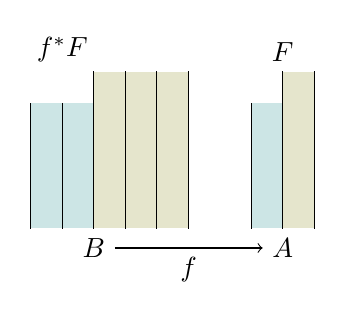
\begin{tikzpicture}
\def\xmin{1.4};
\def\dx{0.4};
\def\xl{-1.4};

\def\dy{0.2};
\def\yb{0};
\def\yt{10 * \dy}; 

% bars over A
\filldraw[fill=blue!50!green!20, draw=white] (\xmin, \yb) rectangle (\xmin + \dx, \yt - 2*\dy);
\filldraw[fill=red!50!green!20, draw=white] (\xmin + \dx, \yb) rectangle (\xmin + 2 * \dx, \yt);

\draw (\xmin, \yb) -- (\xmin, \yt - 2*\dy);
\draw (\xmin + \dx, \yb) -- (\xmin+ \dx, \yt);
\draw (\xmin + 2 * \dx, \yb) -- (\xmin + 2 * \dx, \yt);

\node[below] (BB) at (\xmin + \dx, \yb) {$A$};
\node[above] at (\xmin + \dx, 10 * \dy) {$F$};

% bars over B

\filldraw[fill=blue!50!green!20, draw=white] (\xl, \yb) rectangle (\xl + 5 * \dx, \yt - 2*\dy);
\filldraw[fill=red!50!green!20, draw=white] (\xl + 2*\dx, \yb) rectangle (\xl + 5 * \dx, \yt);
\draw (\xl, \yb) -- (\xl, \yt - 2*\dy);
\draw (\xl + \dx, \yb) -- (\xl + \dx, \yt - 2 * \dy);
\draw (\xl + 2 * \dx, \yb) -- (\xl + 2 * \dx, \yt);
\draw (\xl + 3 * \dx, \yb) -- (\xl + 3 * \dx, \yt);
\draw (\xl + 4 * \dx, \yb) -- (\xl + 4 * \dx, \yt);
\draw (\xl + 5 * \dx, \yb) -- (\xl + 5 * \dx, \yt);

\node[below] (B) at (\xl + 2 * \dx, \yb) {$B$};
\node[above] at (\xl + \dx, 10 * \dy) {$f^* F$};

\draw[->]  (B) -- (BB) node [midway, below] {$f$};


\end{tikzpicture}
\]
$S$ 本身以两种方式纤维化:使用 $f \circ q$ 在 $A$ 上粗切,使用 $q$ 在 $B$ 上细切。

在范畴论中,依赖和是基变换函子 $f^*$ 的左伴随,记为 $f_!$。对于给定的 $f \colon b \to a$,它是一个函子:
\[ f_! \colon \cat C/b \to \cat C/a \]
它对对象 $(s, q \colon s \to b)$ 的作用是通过 $f$ 的后复合给出的:
\[ f_! (s, q)= (s, f \circ q) \]

\subsection{存在量化 (Existential Quantification)}

在\emph{命题作为类型}的解释中,类型族对应于命题族。依赖和类型 $\Sigma_{x : B} \, T(x)$ 对应于命题:存在一个 $x$ 使得 $T(x)$ 为真:
\[ \exists_{x : B} \, T (x)\]

确实,类型 $\Sigma_{x : B} \, T(x)$ 的一个项是一对元素 $x \colon B$ 和 $y \colon T(x)$——这表明对于某个 $x$,$T(x)$ 是可居的(inhabited)。

\section{Dependent Product}

In type theory, the dependent product, or dependent function, or pi-type $\Pi_{x:B} T(x)$, is defined as a function whose return \emph{type} depends on the \emph{value} of its argument. 

It's called a function, because you can evaluate it. Given a dependent function  $f \colon \Pi_{x:B} T(x)$, you may apply it to an argument $x\colon B$ to get a value $f(x) \colon T(x)$.

\subsection{Dependent product in Haskell}
A simple example of a dependent product is a function that constructs a vector of a given size and fills it with copies of a given value:
\begin{haskell}
replicateV :: a -> SNat n -> Vec n a
replicateV _ SZ  = VNil
replicateV x (SS n) = VCons x (replicateV x n)
\end{haskell}

At the time of this writing, Haskell's support for dependent types is limited, so the implementation of dependent functions requires the use of singleton types. In this case, the number that is the argument to \hask{replicateV} is passed as a singleton natural:
\begin{haskell}
data SNat n where
  SZ :: SNat Z
  SS :: SNat n -> SNat (S n)
\end{haskell}
(Note that \hask{replicateV} is a function of two arguments, so it can be either considered a dependent function of a pair, or a regular function returning a dependent function.)
\subsection{Dependent product of sets}
Before we describe the categorical model of dependent functions, it's instructive to consider how they work on sets. A dependent function selects one element from each set $T(x)$. 

You may visualize the totality of this selection as a giant tuple---an element of a cartesian product. For instance, in the trivial case of $B$ a two-element set $\{1, 2\}$, a dependent function type is just a cartesian product $T(1) \times T(2)$. In general, you get one tuple component per every value of $x$. It's a giant tuple indexed by elements of $B$. This is the meaning of the product notation, $\Pi_{x:B} T(x)$. 

In our example, \hask{replicateV} picks a particular counted vector for each value of \hask{n}. Counted vectors are equivalent to tuples so, for \hask{n} equal zero, \hask{replicateV} returns an empty tuple \hask{()}; for \hask{n = 1} it returns a single value \hask{x}; for \hask{n} equal two, it duplicates \hask{x} returning \hask{(x, x)}; etc. 

The function \hask{replicateV}, evaluated at some \hask{x :: a},  is equivalent to an infinite tuple of tuples:
\[ ((), x, (x, x), (x, x, x), ...) \]
which is a specific element of the type:
\[ ((), a, (a, a), (a, a, a), ...) \]

\subsection{Dependent product categorically}
In order to build a categorical model of dependent functions, we need to change our perspective from a family of types to a fibration. We start with a bundle $E/B$ fibered by the projection $p\colon E \to B$. A dependent function is called a \emph{section} of this bundle. 

If you visualize the bundle as a bunch of fibers sticking out from the base $B$, a section is like a haircut: it cuts through each fiber to produce a corresponding value. In physics, such sections are called fields---with spacetime as the base. 

Just like we talked about a function object representing a set of functions, we can talk about an object $S(E)$ that represents a set of sections of a given bundle $E$. 

Just like we defined function application as a mapping out of the product:
\[\varepsilon_{B C} \colon C^B \times B \to C\]
we can define the dependent function application as a mapping:
\[\varepsilon \colon S(E) \times B \to E\]
We can visualize it as picking a section $s$ in $S(E)$ and an element $x$ of the base $B$ and producing a value in the bundle $E$. (In physics, this would correspond to measuring a field at a particular point in spacetime.)

But this time we have to insist that this value be in the correct fiber. If we project the result of applying $\varepsilon$ to $(s, x)$, it should fall back to the $x$. 

\[
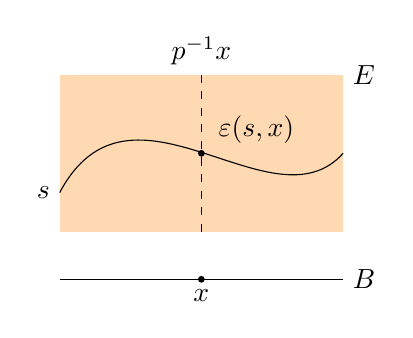
\begin{tikzpicture}

\def\dy{0.2};
\def\yb{-0.6}; % base
\def\yfb{0}; % fiber bottom
\def\yfs{0.5}; % s
\def\yfss{1.0}; % s'
\def\yft{2}; % fiber top

\def\dx{0.9};

\def\xbl{0};
\def\xbmr{\xbl + 2*\dx};
\def\xbr{\xbl + 4*\dx};

\filldraw[fill=orange!30, draw=white] (\xbl, \yfb) rectangle (\xbr, \yft);

\draw (\xbl, \yfb+0.5) .. controls (\xbl + \dx, \yfb + 2.2) and (\xbl + 3* \dx, \yfb) .. (\xbr, \yfb + 1);
\filldraw[black] (\xbmr, \yfb + 1) circle (1 pt);
\node[ above] at (\xbmr + 0.7, \yfb + 1) {$\varepsilon(s, x)$};
\node[left] at  (\xbl, \yfb+0.5) {$s$};
\draw (\xbl, \yb) -- (\xbr, \yb);

\draw[dashed] (\xbmr, \yfb) -- (\xbmr, \yft); %fiber


\filldraw[black] (\xbmr, \yb) circle (1 pt);
\node[below] at (\xbmr, \yb) {$x$};

\node[above] at (\xbmr, \yft) {$p^{-1} x$};

\node[right] at (\xbr, \yb) {$B$};
\node[right] at (\xbr, \yft) {$E$};

\end{tikzpicture}
\]
In other words, this diagram must commute:
\[
 \begin{tikzcd}
 S(E) \times B 
 \arrow[rr, "\varepsilon"]
 \arrow[dr, "\pi_2"']
 && E
 \arrow[dl, "p"]
 \\
 &B
  \end{tikzcd}
\]
This makes $\varepsilon$ a morphism in the slice category $\mathcal{C}/B$.

And just like the exponential object was universal, so is the object of sections. The universality condition has the same form: For any other object $G$ with an arrow $\phi \colon G \times B \to E$ there is a unique arrow $\phi^T \colon G \to S(E)$ that makes the following diagram commute:
\[
 \begin{tikzcd}
 G \times B
 \arrow[d, dashed, "\phi^T \times B"']
 \arrow[dr, "\phi"]
 \\
 S(E) \times B
 \arrow[r, "\varepsilon"]
 &E
  \end{tikzcd}
\]
The difference is that both $\varepsilon$ and $\phi$ are now morphisms in the slice category $\mathcal{C}/B$. 

The one-to-one correspondence between $\phi$ and $\phi^T$ forms the adjunction:
\[(\mathcal{C}/B) \left( \left \langle {G\times B \atop \pi_2} \right \rangle , \left \langle {E \atop p } \right \rangle \right) \cong \mathcal{C} \left(G, S(E)\right) \]
which we can use as the definition of the object of sections $S(E)$. The counit of this adjunction is  the dependent-function application. We get it by replacing $G$ with $S(E)$ and selecting the identity morphism on the right. The counit is thus a member of the hom-set:
\[(\mathcal{C}/B) \left( \left \langle {S(E) \times B \atop \pi_2} \right \rangle , \left \langle {E \atop p } \right \rangle \right) \]


Compare the above adjunction with the currying adjunction that defines the function object $E^B$:
\[  \cat C (G \times B, E) \cong \cat C (G, E^B) \]

Now recall that, in $\mathbf{Set}$, we interpret the product $G \times B$ as planting copies of $G$ as identical fibers over each element of $B$.  So a single element of the left-hand side of our adjunction is a family of functions, one per fiber. Any given $y \in G$ cuts a horizontal slice through $G \times B$. These are the pairs $(y, b)$ for all $b \in B$. Our family of functions maps this slice to the corresponding fibers of $E$ thus creating a section of $E$.

\[
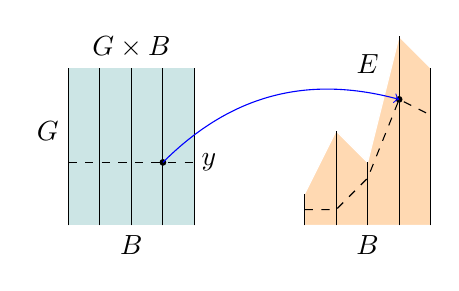
\begin{tikzpicture}
\def\dy{0.2};
\def\yb{0};
\def\yt{10 * \dy}; 

\def\dx{0.4};
\def\xl{-2};
\def\xr{1};

\filldraw[fill=blue!50!green!20, draw=white] (\xl, \yb) rectangle (\xl + 4 * \dx, \yt);
\draw (\xl, \yb) -- (\xl, \yt);
\draw (\xl + \dx, \yb) -- (\xl + \dx, \yt);
\draw (\xl + 2 * \dx, \yb) -- (\xl + 2 * \dx, \yt);
\draw (\xl + 3 * \dx, \yb) -- (\xl + 3 * \dx, \yt);
\draw (\xl + 4 * \dx, \yb) -- (\xl + 4 * \dx, \yt);
\node[below] at (\xl + 2 * \dx, \yb) {$B$};
\node[left] at (\xl + 5 * \dx,  4 * \dy) {$y$};
\node[left] at (\xl,  6 * \dy) {$G$};
\node[above] at (\xl + 2*\dx, 10 * \dy) {$G \times B$};

\def\a{2* \dy}
\def\b{6* \dy}
\def\c{4* \dy}
\def\d{12* \dy}
\def\e{10* \dy}


\draw[fill=orange!30, draw=white] (\xr, \yb) -- (\xr, \a) -- (\xr + 1 * \dx, \b) -- (\xr + 2 * \dx, \c) -- (\xr + 3 * \dx, \d) -- (\xr + 4 * \dx, \e) -- (\xr + 4 * \dx, \yb) -- cycle;


\draw (\xr, \yb) -- (\xr, \a);
\draw (\xr + \dx, \yb) -- (\xr + \dx, \b);
\draw (\xr + 2 * \dx, \yb) -- (\xr + 2 * \dx, \c);
\draw (\xr + 3 * \dx, \yb) -- (\xr + 3 * \dx, \d);
\draw (\xr + 4 * \dx, \yb) -- (\xr + 4 * \dx, \e);

\node[below] at (\xr + 2 * \dx, \yb) {$B$};
\node[above] at (\xr + 2 * \dx, 9 * \dy) {$E$};

\draw[dashed] (\xr, \a -\dy ) -- (\xr + 1 * \dx, \b - 5 * \dy) -- (\xr + 2 * \dx, \c - \dy) -- (\xr + 3 * \dx, \d - 4*\dy) -- (\xr + 4 * \dx, \e - 3*\dy);


\filldraw[black] (\xl + 3 * \dx, \yb + 4* \dy) circle (1 pt);
\filldraw[black] (\xr + 3 * \dx, \yb + 8* \dy) circle (1 pt);

\draw[blue] ((\xl + 3 * \dx, \yb + 4* \dy) edge[->, bend left] (\xr + 3 * \dx, \yb + 8* \dy);

\draw[dashed] (\xl, \yb + 4* \dy) -- (\xl + 4* \dx, \yb + 4* \dy);

\end{tikzpicture}
\]

The adjunction tells us that this family of mappings uniquely determines a function from $G$ to $S(E)$. Every $y \in G$ is thus mapped to a different element $s$ of $S(E)$. Therefore elements of $S(E)$ are in one-to-one correspondence with sections of $E$ .

These are all set-theoretical intuitions. We can generalize them by first noticing that the right hand side of the adjunction can be easily expressed as a hom-set in the slice category $\mathcal{C}/1$ over the terminal object. 

Indeed, there is one-to-one correspondence between objects $X$ in $\mathcal{C}$ and objects $\langle X, ! \rangle$ in  $\mathcal{C}/1$ (here $!$ is the unique arrow to the terminal object). Arrows in $\mathcal{C}/1$ are arrows of $\mathcal{C}$ with no additional constraints. We therefore have:
\[(\mathcal{C}/B) \left( \left \langle {G\times B \atop \pi_2} \right \rangle , \left \langle {E \atop p } \right \rangle \right) \cong (\mathcal{C}/1)  \left( \left \langle {G \atop !} \right \rangle , \left \langle {S(E) \atop ! } \right \rangle \right)  \]

\subsection{Adding the atlas}

The next step is to ``blur the focus'' by replacing the terminal object with a more general base $A$, serving as the atlas.

The right-hand side of the adjunction becomes a hom-set in the slice category $\mathcal{C}/A$. $G$ itself gets coarsely fibrated by some $q \colon G \to A$. 

Remember that $G \times B$ can be understood as a pullback along the mapping $! \colon B \to 1$, or a change of base from $1$ to $B$. If we want to replace $1$ with $A$, we should replace the product $G \times B$ with a more general pullback of $q$. Such a change of base is parameterized by a new morphism $f \colon B \to A$.

\[
 \begin{tikzcd}
 G \times B
 \arrow[dr, phantom,  , very near start, "\lrcorner"]
\arrow[d, "\pi_2"]
 \arrow[r, "\pi_1"]
 & G
 \arrow[d, "!"]
 \\
 B
 \arrow[r, "!"]
 &
 1
 \end{tikzcd}
 \hspace{20pt}
\begin{tikzpicture}
\draw[->] (0, 0) -- (1, 0);
\end{tikzpicture}
 \hspace{20pt}
 \begin{tikzcd}
 f^* G
\arrow[dr, phantom,  , very near start, "\lrcorner"]
 \arrow[d, "f^*q"']
 \arrow[r, "g"]
 & G
 \arrow[d, "q"]
 \\
 B
 \arrow[r, "f"]
 &A
\end{tikzcd}
\]

The result is that, instead of a bunch of $G$ fibers over $B$, we get a pullback $f^* G$ that is populated by groups of fibers from the fibration $q \colon G \to A$. This way $A$ serves as an atlas that enumerates all the patches populated by uniform fibers. 

Imagine, for instance, that $A$ is a two-element set. The fibration $q$ will split $G$ into two fibers. They will serve as our generic fibers. These fibers are now replanted over the two patches in $B$ to form $f^* G$. The replanting is guided by $f^{-1}$. 

\[
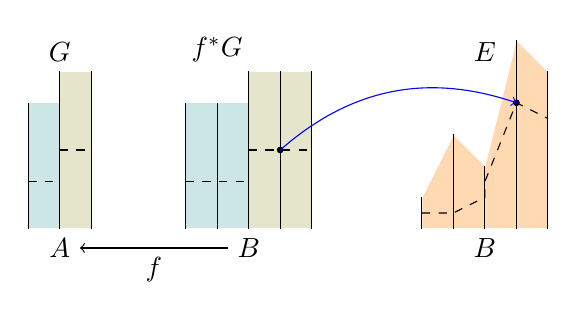
\begin{tikzpicture}
\def\xmin{-4};

\def\dy{0.2};
\def\yb{0};
\def\yt{10 * \dy}; 

\def\dx{0.4};
\def\xl{-2};
\def\xr{1};

\filldraw[fill=blue!50!green!20, draw=white] (\xmin, \yb) rectangle (\xmin + \dx, \yt - 2*\dy);
\filldraw[fill=red!50!green!20, draw=white] (\xmin + \dx, \yb) rectangle (\xmin + 2 * \dx, \yt);
\draw (\xmin, \yb) -- (\xmin, \yt - 2*\dy);
\draw (\xmin + \dx, \yb) -- (\xmin+ \dx, \yt);
\draw (\xmin + 2 * \dx, \yb) -- (\xmin + 2 * \dx, \yt);
\node[below] (BB) at (\xmin + \dx, \yb) {$A$};
\node[above] at (\xmin + \dx, 10 * \dy) {$G$};



\filldraw[fill=blue!50!green!20, draw=white] (\xl, \yb) rectangle (\xl + 4 * \dx, \yt - 2*\dy);
\filldraw[fill=red!50!green!20, draw=white] (\xl + 2 * \dx, \yb) rectangle (\xl + 4 * \dx, \yt);
\draw (\xl + 0 * \dx, \yb) -- (\xl + 0 * \dx, \yt - 2 * \dy);
\draw (\xl + 1 * \dx, \yb) -- (\xl + 1 * \dx, \yt - 2 * \dy);
\draw (\xl + 2 * \dx, \yb) -- (\xl + 2 * \dx, \yt);
\draw (\xl + 3 * \dx, \yb) -- (\xl + 3 * \dx, \yt);
\draw (\xl + 4 * \dx, \yb) -- (\xl + 4 * \dx, \yt);
\node[below] (B) at (\xl + 2 * \dx, \yb) {$B$};
\node[above] at (\xl + \dx, 10 * \dy) {$f^* G$};

\draw[->]  (B) -- (BB) node [midway, below] {$f$};

\def\a{2* \dy}
\def\b{6* \dy}
\def\c{4* \dy}
\def\d{12* \dy}
\def\e{10* \dy}


\draw[fill=orange!30, draw=white] (\xr, \yb) -- (\xr, \a) -- (\xr + 1 * \dx, \b) -- (\xr + 2 * \dx, \c) -- (\xr + 3 * \dx, \d) -- (\xr + 4 * \dx, \e) -- (\xr + 4 * \dx, \yb) -- cycle;


\draw (\xr, \yb) -- (\xr, \a);
\draw (\xr + \dx, \yb) -- (\xr + \dx, \b);
\draw (\xr + 2 * \dx, \yb) -- (\xr + 2 * \dx, \c);
\draw (\xr + 3 * \dx, \yb) -- (\xr + 3 * \dx, \d);
\draw (\xr + 4 * \dx, \yb) -- (\xr + 4 * \dx, \e);

\node[below] at (\xr + 2 * \dx, \yb) {$B$};
\node[above] at (\xr + 2 * \dx, 10 * \dy) {$E$};

% dashed zigzag in E
\draw[dashed] (\xr, \a -\dy ) -- (\xr + 1 * \dx, \b - 5 * \dy) -- (\xr + 2 * \dx, \c - 2* \dy)  -- (\xr + 2 * \dx, \c - \dy) -- (\xr + 3 * \dx, \d - 4*\dy) -- (\xr + 4 * \dx, \e - 3*\dy);

\filldraw[black] (\xl + 3 * \dx, \yb + 5* \dy) circle (1 pt);
\filldraw[black] (\xr + 3 * \dx, \yb + 8* \dy) circle (1 pt);

% arrow from f*G to E
\draw[blue] ((\xl + 3 * \dx, \yb + 5* \dy) edge[->, bend left] (\xr + 3 * \dx, \yb + 8* \dy);

% dashed slices through f*G
\draw[dashed] (\xl, \yb + 3* \dy) -- (\xl + 2 * \dx, \yb + 3* \dy);
\draw[dashed] (\xl + 2 * \dx, \yb + 5* \dy) -- (\xl + 4* \dx, \yb + 5* \dy);

% slices through G
\draw[dashed] (\xmin, \yb + 3* \dy) -- (\xmin + \dx, \yb + 3* \dy);
\draw[dashed] (\xmin + \dx, \yb + 5* \dy) -- (\xmin + 2 * \dx, \yb + 5* \dy);

\end{tikzpicture}
\]

The adjunction that defines the dependent function type is therefore:
\[ (\mathcal{C}/B) \left( f^* \left \langle {G \atop q} \right \rangle, \left \langle {E \atop p} \right \rangle \right) \cong  (\mathcal{C}/A)\left( \left \langle {G \atop q} \right \rangle, \Pi_f \left \langle {E \atop p } \right \rangle \right) \]
This is a generalization of an adjunction that we used to define the object of sections $S(E)$. This one defines a new object $\Pi_f E$ that is a rearrangement of the object of sections. 

The adjunction is a mapping between morphisms in their respective slice categories:

\[
 \begin{tikzcd}
 f^* G
 \arrow[rr, "\phi"]
 \arrow[rd, "f^* q"']
 &&E
 \arrow[dl, "p"]
 \\
 &B
 \end{tikzcd}
 \hspace{20pt}
\begin{tikzcd}
 G
 \arrow[rr, "\phi^T"]
 \arrow[rd, "q"']
 && \Pi_f E
 \arrow[ld, "\Pi_f \, p"]
 \\
 & A
  \end{tikzcd}
\]

To gain some intuition into this adjunction, let's consider how it works on sets. 

\begin{itemize}
\item The right hand side operates in a coarsely grained fibration over the atlas $A$. It is a family of functions, one function per patch. For every patch we get a function from the ``thick fiber'' of $G$ (drawn in blue below) to the ``thick fiber'' of $\Pi_f E$ (not shown).

\item The left hand side operates in a more finely grained fibration over $B$. These fibers are grouped into small bundles over patches. Once we pick a patch (drawn in red below), we get a family of functions from that patch to the corresponding patch in $E$ (drawn in green)---a section of a small bundle in $E$. So, patch-by-patch, we get small sections of $E$. 
\end{itemize}
The adjunction tells us that the elements of the ``thick fiber'' of $\Pi_f E$ correspond to small sections of $E$ over the same patch.

\[
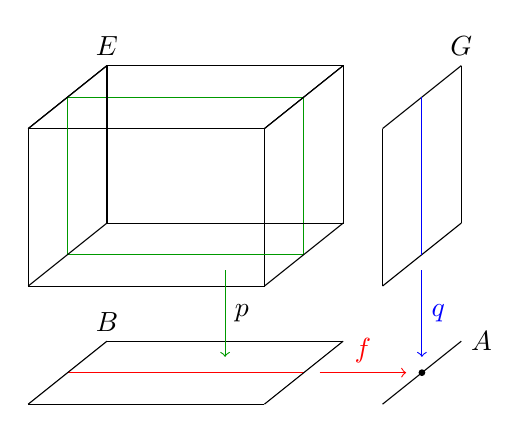
\begin{tikzpicture}
\def\xl{-3};
\def\xr{0};
\def\yb{0};
\def\yt{2};

\def\dy{0.4};
\def\dx{0.5};

\def\a{(\xl, \yb)};
\def\b{(\xr, \yb)};
\def\c{(\xl, \yt)};
\def\d {(\xr, \yt)};

% _a second plane
\def\aa{(\xl + \dx, \yb + \dy)};
\def\ba{(\xr + \dx, \yb + \dy)};
\def\ca{(\xl + \dx, \yt + \dy)};
\def\da{(\xr + \dx, \yt + \dy)};

% _b third plane
\def\ab{(\xl + 2*\dx, \yb + 2*\dy)};
\def\bb{(\xr + 2*\dx, \yb + 2*\dy)};
\def\cb{(\xl + 2*\dx, \yt + 2*\dy)};
\def\db{(\xr + 2*\dx, \yt + 2*\dy)};

% shifted walls
\def\yshift{-1.5};
\def\xshift{1.5};


% E
\draw \a rectangle \d;
\draw[draw=black!40!green] \aa rectangle \da;
\draw \ab rectangle \db;

\draw \a -- \ab;
\draw \b -- \bb;
\draw \d -- \db;
\draw \c -- \cb;

\node[above] at \cb {$E$};

% B
% rebase yb (bottom)
\def\yb{\yshift}
% rebase xr (right wall)
\def\xr{0};

\draw \a -- \b;
\draw \ab -- \bb;
\draw[red] \aa -- \ba;
% diagonal
\draw \a -- \ab;
\draw \b -- \bb;
\draw \d -- \db;
\draw \c -- \cb;
\node[above] at \ab {$B$};

% G
% rebase yb (bottom)
\def\yb{0};
% rebase xr (right wall)
\def\xr{\xshift};
\draw \b -- \bb;
\draw \d -- \db;
\draw \b -- \d;
\draw \bb -- \db;
\draw[blue] \ba -- \da;
\node[above] at \db {$G$};

% A
% rebase yb (bottom)
\def\yb{\yshift}
% rebase xr (right wall)
\def\xr{\xshift};

\draw \b -- \bb;
\node[right] at \bb {$A$};
\filldraw[black] \ba circle (1 pt);

%projections
\draw[blue, shorten <=0.2cm, shorten >=0.2cm, ->] (\xshift + \dx, 0 + \dy) -- node[right]{$q$} (\xshift +\dx, \yshift + \dy);

\draw[red, shorten <=0.2cm, shorten >=0.2cm, ->] (0 + \dx, \yshift + \dy) -- node[above]{$f$} (\xshift +\dx, \yshift + \dy);

\draw[draw=black!40!green, shorten <=0.2cm, shorten >=0.2cm, ->] (0 - \dx, 0 + \dy) -- node[right]{$p$} (0 - \dx, \yshift + \dy);

\end{tikzpicture}
\]

In category theory, the dependent product, which is the right adjoint to the base change functor $f^*$, is denoted by $f_*$. For a given $f \colon b \to a$, it's a functor:
\[ f_* \colon \cat C/b \to \cat C/a \]

The following exercises shed some light on the role played by $f$. It can be seen as localizing the sections of $E$ by restricting them to ``neighborhoods'' defined by $f^{-1}$.

\begin{exercise}
Consider what happens when $A$ is a two-element set $\{0, 1\}$ and $f$ maps the whole of $B$ to one element, say $1$. How would you define the function on the right-hand side of the adjunction? What should it do to the fiber over $0$?
\end{exercise}

\begin{exercise}
Let's pick $G$ to be a singleton set $1$, and let $x \colon 1 \to A$ be a fibration that selects an element in $A$. Using the adjunction, show that:
\begin{itemize}
\item $f^* 1$ has two types of fibers: singletons over the elements of $f^{-1} (x)$ and empty sets otherwise. 
\item A mapping $\phi \colon f^* 1 \to E$ is equivalent to a selection of elements, one from each fiber of $E$ over the elements of $f^{-1}(x)$. In other words, it's a partial section of $E$ over the subset $f^{-1}(x)$ of $B$.
\item A fiber of $\Pi_f E$ over a given $x$ is such a partial section. 
\item What happens when $A$ is also a singleton set?
\end{itemize}
\end{exercise}



\subsection{Universal quantification}

The logical interpretation of the dependent product $\Pi_{x : B} \, T(x)$ is a universally quantified proposition. An element of $\Pi_{x : B} \, T(x)$ is a section---the proof that it's possible to select an element from each member of the family $T(x)$. It means that none of them is empty. In other words, it's a proof of the proposition:
\[ \forall_{x : B}\, T(x) \]



\section{相等性}

我们在数学中的第一个体验涉及相等性。我们学习到
\[1+1=2\]
之后我们并没有过多思考它。

但是$1+1$等于$2$意味着什么?2是一个数字,但1加1是一个表达式,所以它们不是同一个东西。在我们宣布这两个东西相等之前,我们需要进行一些心理处理。

与此形成对比的是语句$0 = 0$,其中等式的两边是\emph{同一个东西}。

如果我们定义相等性,至少需要确保每个东西都等于它自己,这是有意义的。我们称这个性质为\emph{自反性}。

回顾我们对自然数的定义:
\begin{haskell}
data Nat where
  Z :: Nat
  S :: Nat -> Nat
\end{haskell}

这是我们为自然数定义相等性的方式:
\begin{haskell}
equal :: Nat -> Nat -> Bool
equal Z Z = True
equal (S m) (S n) = equal m n
equal _ _ = False
\end{haskell}
我们递归地剥离每个数字中的$S$,直到其中一个达到$Z$。如果另一个同时达到$Z$,我们宣布我们开始的数字相等,否则它们不相等。

\subsection{等式推理}

注意,在Haskell中定义相等性时,我们已经使用了等号。例如,在以下代码中的等号:
\begin{haskell}
equal Z Z = True
\end{haskell}
告诉我们,无论在哪里看到表达式\hask{equal Z Z},我们都可以用\hask{True}替换它,反之亦然。

这是用等量替换等量的原则,这是Haskell中\emph{等式推理}的基础。我们不能直接在Haskell中编码相等性的证明,但我们可以使用等式推理来推理Haskell程序。这是纯函数式编程的主要优势之一。在命令式语言中,由于副作用,你不能执行这样的替换。

如果我们想证明$1+1$等于$2$,我们必须首先定义加法。定义可以在第一个或第二个参数中递归。这个定义在第二个参数中递归:
\begin{haskell}
add :: Nat -> Nat -> Nat
add n Z = n
add n (S m) = S (add n m)
\end{haskell}
我们将$1 + 1$编码为:
\begin{haskell}
add (S Z) (S Z)
\end{haskell}
我们现在可以使用\hask{add}的定义来简化这个表达式。我们尝试匹配第一个子句,但失败了,因为\hask{S Z}与\hask{Z}不同。但第二个子句匹配。在其中,\hask{n}是一个任意数字,所以我们可以用\hask{S Z}替换它,得到:
\begin{haskell}
add (S Z) (S Z) = S (add (S Z) Z)
\end{haskell}
在这个表达式中,我们可以使用\hask{add}定义的第一个子句(再次用\hask{S Z}替换\hask{n})进行另一个等量替换:
\begin{haskell}
add (S Z) Z = (S Z)
\end{haskell}
我们得到:
\begin{haskell}
add (S Z) (S Z) = S (S Z)
\end{haskell}
我们可以清楚地看到右边是$2$的编码。但我们还没有证明我们的相等性定义是自反的,所以原则上我们不知道
\begin{haskell}
eq (S (S Z)) (S (S Z))
\end{haskell}
是否产生\hask{True}。我们必须再次使用逐步的等式推理:
\begin{haskell}
equal (S (S Z) (S (S Z)) =
{- 相等性定义的第二个子句 -}
equal (S Z) (S Z) =
{- 相等性定义的第二个子句 -}
equal Z Z =
{- 相等性定义的第一个子句 -}
True
\end{haskell}

我们可以使用这种推理来证明关于具体数字的陈述,但在推理通用数字时会遇到问题——例如,证明某个东西对所有\hask{n}都成立。使用我们的加法定义,我们可以很容易地证明\hask{add n Z}与\hask{n}相同。但我们不能证明\hask{add Z n}与\hask{n}相同。后者的证明需要使用归纳法。

我们最终区分了两种相等性。一种是通过替换或重写规则证明的,称为\emph{定义相等性}。你可以将其视为编程语言中的宏扩展或内联扩展。它还涉及$\beta$-归约:通过用实际参数替换形式参数来执行函数应用,如:
\begin{haskell}
(\x -> x + x) 2 =
{- beta 归约 -}
2 + 2
\end{haskell}

第二种更有趣的相等性称为\emph{命题相等性},它可能需要实际的证明。

\subsection{相等性与同构}

我们说范畴论者更喜欢同构而不是相等性——至少在对象方面是这样。确实,在范畴的范围内,无法区分同构的对象。但一般来说,相等性比同构更强。这是一个问题,因为能够用等量替换等量非常方便,但并不总是清楚是否可以用同构替换同构。

数学家们一直在努力解决这个问题,主要是试图修改同构的定义——但当他们决定同时弱化相等性的定义时,真正的突破出现了。这导致了\emph{同伦类型论}(Homotopy Type Theory,简称HoTT)的发展。

粗略地说,在类型论中,特别是在Martin-L{\"o}f的依赖类型理论中,相等性被表示为一个类型,为了证明相等性,必须构造该类型的一个元素——这是Curry-Howard解释的精神。

此外,在HoTT中,证明本身可以比较相等性,依此类推,无限进行。你可以通过将相等性的证明视为一些可以相互变形的抽象路径来想象这一点;因此使用了同伦的语言。

在这种设置中,不是使用涉及箭头的严格相等性的同构:
\[ f \circ g = id \]
\[ g \circ f = id \]
而是定义一个\emph{等价性},其中这些相等性被视为类型。

HoTT的主要思想是可以施加\emph{单值公理},粗略地说,它声明相等性等价于等价性,或符号化地:
\[ (A = B) \cong (A \cong B) \]
注意,这是一个公理,而不是定理。我们可以接受它或放弃它,理论仍然有效(至少我们这么认为)。

\subsection{相等性类型}

假设你想比较两个项是否相等。第一个要求是这两个项必须是同一类型。你不能比较苹果和橙子。不要被一些编程语言允许比较不同类型的项所迷惑:在每种情况下,都涉及隐式转换,最终的相等性总是在相同类型的值之间。

原则上,对于每一对值,都有一个单独的相等性证明类型。有$0 = 0$的类型,有$1=1$的类型,还有$1 = 0$的类型;后者希望是无人居住的。

相等性类型,也称为恒等类型,因此是一个依赖类型:它取决于我们正在比较的两个值。它通常写为$\text{Id}_A$,其中$A$是两个值的类型,或者使用中缀符号写为$x=_A y$(等号带有下标$A$)。

例如,两个零的相等性类型写为$\text{Id}_{\mathbb{N}} (0, 0)$或:
\[ 0 =_{\mathbb{N}} 0 \]
注意:这不是一个语句或一个项。它是一个\emph{类型},如\hask{Int}或\hask{Bool}。如果你有它的引入规则,你可以定义该类型的一个值。

\subsection{引入规则}

相等性类型的引入规则是依赖函数:
\[ \text{refl}_A \colon \Pi_{x : A}  \text{Id}_A  (x, x)\]
它可以被解释为命题即类型的精神,作为以下语句的证明:
\[ \forall _{x:A} \;x = x \]
这是熟悉的自反性:它表明,对于所有类型为$A$的$x$,$x$等于它自己。你可以将此函数应用于类型为$A$的某个具体值$x$,它将产生一个类型为$\text{Id}_A  (x, x)$的新值。

我们现在可以证明$0=0$。我们可以执行$\text{refl}_{\mathbb{N}} (0)$来获得类型$0 =_{\mathbb{N}} 0$的一个值。这个值是该类型被居住的证明,因此对应于一个真命题。

这是相等性的唯一引入规则,所以你可能会认为所有相等性的证明都归结为“它们相等,因为它们是相同的。”令人惊讶的是,事实并非如此。

\subsection{$\beta$-归约和$\eta$-转换}

在类型论中,我们有引入和消除规则的相互作用,这本质上使它们互为逆。

考虑积的定义。我们通过提供两个值$x \colon A$和$y \colon B$来引入它,并得到一个值$p \colon A \times B$。然后我们可以通过使用两个投影提取两个值来消除它。但我们如何知道这些是否是我们用来构造它的相同值?这是我们必须假设的东西。我们称之为计算规则或$\beta$-归约规则。

相反,如果我们给定一个值$p \colon A \times B$,我们可以使用投影提取两个分量,然后使用引入规则重新组合它。但我们如何知道我们会得到相同的$p$?这也必须假设。这有时被称为唯一性条件,或$\eta$-转换规则。

在类型论的范畴模型中,这两个规则遵循普遍构造。

相等性类型也有消除规则,我们稍后会讨论,但我们不施加唯一性条件。这意味着可能存在一些不是通过$\text{refl}$获得的相等性证明。

这正是使HoTT对数学家感兴趣的相等性概念的弱化。

\subsection{自然数的归纳原理}

在制定相等性的消除规则之前,先讨论一个更简单的自然数的消除规则是有益的。我们已经看到了描述原始递归的规则。它允许我们通过指定一个值$\mathit{init}$和一个函数$\mathit{step}$来定义递归函数。

使用依赖类型,我们可以将此规则推广为定义\emph{依赖消除规则},它等价于数学归纳原理。

归纳原理可以被描述为一种设备,用于一举证明由自然数索引的整个命题族。例如,语句\hask{add Z n}等于\hask{n}实际上是一个无限数量的命题,每个\hask{n}的值对应一个。

原则上,我们可以编写一个程序,仔细验证这个语句在大量情况下的正确性,但我们永远无法确定它是否普遍成立。有一些关于自然数的猜想已经通过计算机以这种方式进行了测试,但显然,它们永远无法穷尽无限的情况。

粗略地说,我们可以将所有数学定理分为两组:易于表述的和表述复杂的。它们可以进一步细分为证明简单的和难以或无法证明的。例如,著名的费马大定理非常容易表述,但其证明需要一些极其复杂的数学工具。

在这里,我们感兴趣的是那些既易于表述又易于证明的关于自然数的定理。我们假设我们知道如何生成一个命题族,或者等价地,一个依赖类型$T(n)$,其中$n$是一个自然数。

我们还假设我们有一个值:
\[\mathit{init} \colon T(Z) \]
或者等价地,第零个命题的证明;以及一个依赖函数:
\[\mathit{step} \colon \Pi_{n:\mathbb{N}}\,\left(T(n) \to T(S n)\right) \]
这个函数被解释为从第$n$个命题的证明生成第$(n + 1)$个命题的证明。

自然数的\emph{依赖消除规则}假设,给定这样的$\mathit{init}$和$\mathit{step}$,存在一个依赖函数:
\[f \colon \Pi_{n:\mathbb{N}} \, T(n) \]
这个函数被解释为提供$T(n)$对所有$n$都成立的证明。

此外,这个函数在应用于零时重现$\mathit{init}$:
\[ f (Z) = \mathit{init} \]
并且在应用于$n$的后继时与采取$\mathit{step}$一致:
\[ f (S n) = (\mathit{step} (n)) (f (n)) \]
(在这里,$\mathit{step}(n)$产生一个函数,然后应用于值$f(n)$。)这些是自然数的两个\emph{计算规则}。

注意,归纳原理不是关于自然数的一个定理。它是自然数类型\emph{定义}的一部分。

并非所有从自然数出发的依赖映射都可以分解为$\mathit{init}$和$\mathit{step}$,就像并非所有关于自然数的定理都可以通过归纳法证明一样。自然数没有$\eta$-转换规则。

\subsection{相等性消除规则}

相等性类型的消除规则,也称为\index{J-rule}J-rule,在某种程度上类似于自然数的归纳原理。在那里,我们使用$\mathit{init}$在旅程开始时立足,并使用$\mathit{step}$取得进展。相等性的消除规则需要更强大的立足点,但它没有$\mathit{step}$。除了通过信仰的飞跃,真的没有好的类比来解释它是如何工作的。

其思想是我们想构造一个从相等性类型出发的映射。但由于相等性类型本身是一个双参数类型族,出发的映射应该是一个依赖函数。这个函数的目标是另一个类型族:
\[T(x, y, p)\]
它取决于正在比较的两个值$x, y \colon A$,以及相等性证明$p \colon \text{Id}(x, y)$。

我们试图构造的函数是:
\[ f \colon \Pi_{x, y : A} \Pi_{p : \text{Id}(x, y)} \, T(x, y, p) \]

将其视为生成一个证明是方便的,即对于所有点$x$和$y$,以及对于每两个点相等的证明,命题$T(x, y, p)$为真。注意,潜在情况下,我们对于\emph{每两个点相等的证明}都有一个不同的命题。

我们对$T(x, y, p)$的最低要求是,当$x$和$y$字面上相同,且相等性证明是明显的$\text{refl}$时,它应该为真。这个要求可以表示为一个依赖函数:
\[t \colon \Pi_{x : A} \,T\left(x, x, \text{refl}(x)\right)\]
注意,我们甚至不考虑$x = x$的证明,除了那些由自反性给出的证明。这样的证明存在吗?我们不知道,也不关心。

所以这是我们的立足点,一个旅程的起点,它应该引导我们为所有点对和所有相等性证明定义我们的$f$。直觉是,我们将$f$定义为一个在平面$(x, y)$上的函数,第三个维度由$p$给出。为此,我们得到了在$(x, x)$对角线上定义的东西,$p$限制为$\text{refl}$。

\[
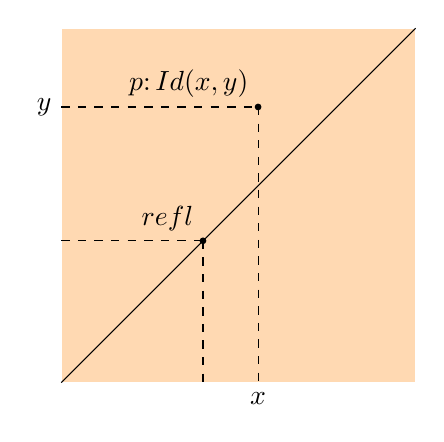
\begin{tikzpicture}

\def\yb{0}; 
\def\ydiag{1.8};
\def\yoff{3.5};
\def\yt{4.5}; 


\def\xl{0};
\def\xdiag{\ydiag};
\def\xoff{2.5};
\def\xr{\yt};

\filldraw[fill=orange!30, draw=white] (\xl, \yb) rectangle (\xr, \yt);

\draw (\xl, \yb) -- (\xr, \yt); % diagonal

\draw[dashed] (\xdiag, \ydiag) -- (\xdiag, \yb);
\draw[dashed] (\xl, \ydiag) -- (\xdiag, \ydiag);

\filldraw[black] (\xdiag, \ydiag) circle (1 pt);
\node[above left] at (\xdiag, \ydiag) {$\text{refl}$};

\draw[dashed] (\xoff, \yoff) -- (\xoff, \yb);
\draw[dashed] (\xl, \yoff) -- (\xoff, \yoff);

\filldraw[black] (\xoff, \yoff) circle (1 pt);
\node[above left] at (\xoff, \yoff) {$p\colon \text{Id}(x, y)$};

\node[below] at (\xoff, \yb) {$x$};
\node[left] at (\xl, \yoff) {$y$};

\end{tikzpicture}
\]

你可能会认为我们需要更多的东西,某种$\mathit{step}$,可以将我们从一点移动到另一点。但与自然数不同,没有\emph{下一个}点或\emph{下一个}相等性证明可以跳转。我们手头只有函数$t$,没有其他东西。

因此我们假设,给定一个类型族$T(x, y, p)$和一个函数:
\[t \colon \Pi_{x : A} \,T\left(x, x, \text{refl}(x)\right)\]
存在一个函数:
\[ f \colon \Pi_{x, y : A} \Pi_{p : \text{Id}(x, y)} \, T(x, y, p) \]
使得(计算规则):
\[f (x, x, \text{refl}(x)) = t(x)\]
注意,计算规则中的相等性是\emph{定义相等性},而不是一个类型。

相等性消除告诉我们,总是可以将定义在对角线上的函数$t$扩展到整个三维空间。

这是一个非常强的假设。理解它的一种方式是,在类型论的框架内——它是使用引入和消除规则以及操作这些规则的语言制定的——\emph{不可能}定义一个不满足相等性消除规则的类型族$T(x, y, p)$。

我们迄今为止看到的最接近的类比是参数化的结果,它表明,在Haskell中,所有在自函子之间的多态函数自动是自然变换。另一个例子,这次来自微积分,是任何在实轴上定义的分析函数都有唯一的扩展到整个复平面。

依赖类型的使用模糊了编程和数学之间的界限。有一系列语言,从Haskell刚刚涉足依赖类型,但仍然牢固地建立在商业使用中,一直到帮助数学家形式化数学证明的定理证明器。

\end{document}